\documentclass{standalone}

\usepackage{pgfplots}
\usepackage{tikz}
\usetikzlibrary{shapes,arrows,positioning}

% Tikzstyles and commands
\tikzstyle{decision} = [diamond, aspect=2, draw, fill=green!20, minimum size=7mm, node distance=2cm]
\tikzstyle{block} = [rectangle, draw, fill=blue!20, minimum size=7mm, node distance=1.5cm]
\tikzstyle{arrow} = [draw, thick, color=black!50, ->]
\tikzstyle{line} = [draw, thick, color=black!50, -]
\tikzstyle{cloud} = [draw, ellipse,fill=red!20, minimum size=7mm, node distance=1.5cm]
\tikzstyle{answer}=[near start,color=black]
\tikzstyle{fake}=[inner sep=0cm, line width=0mm, fill=black!50, radius={\pgflinewidth}]
\tikzstyle{point}=[inner sep=0.5mm, line width=0mm, shape=circle]

\begin{document}

 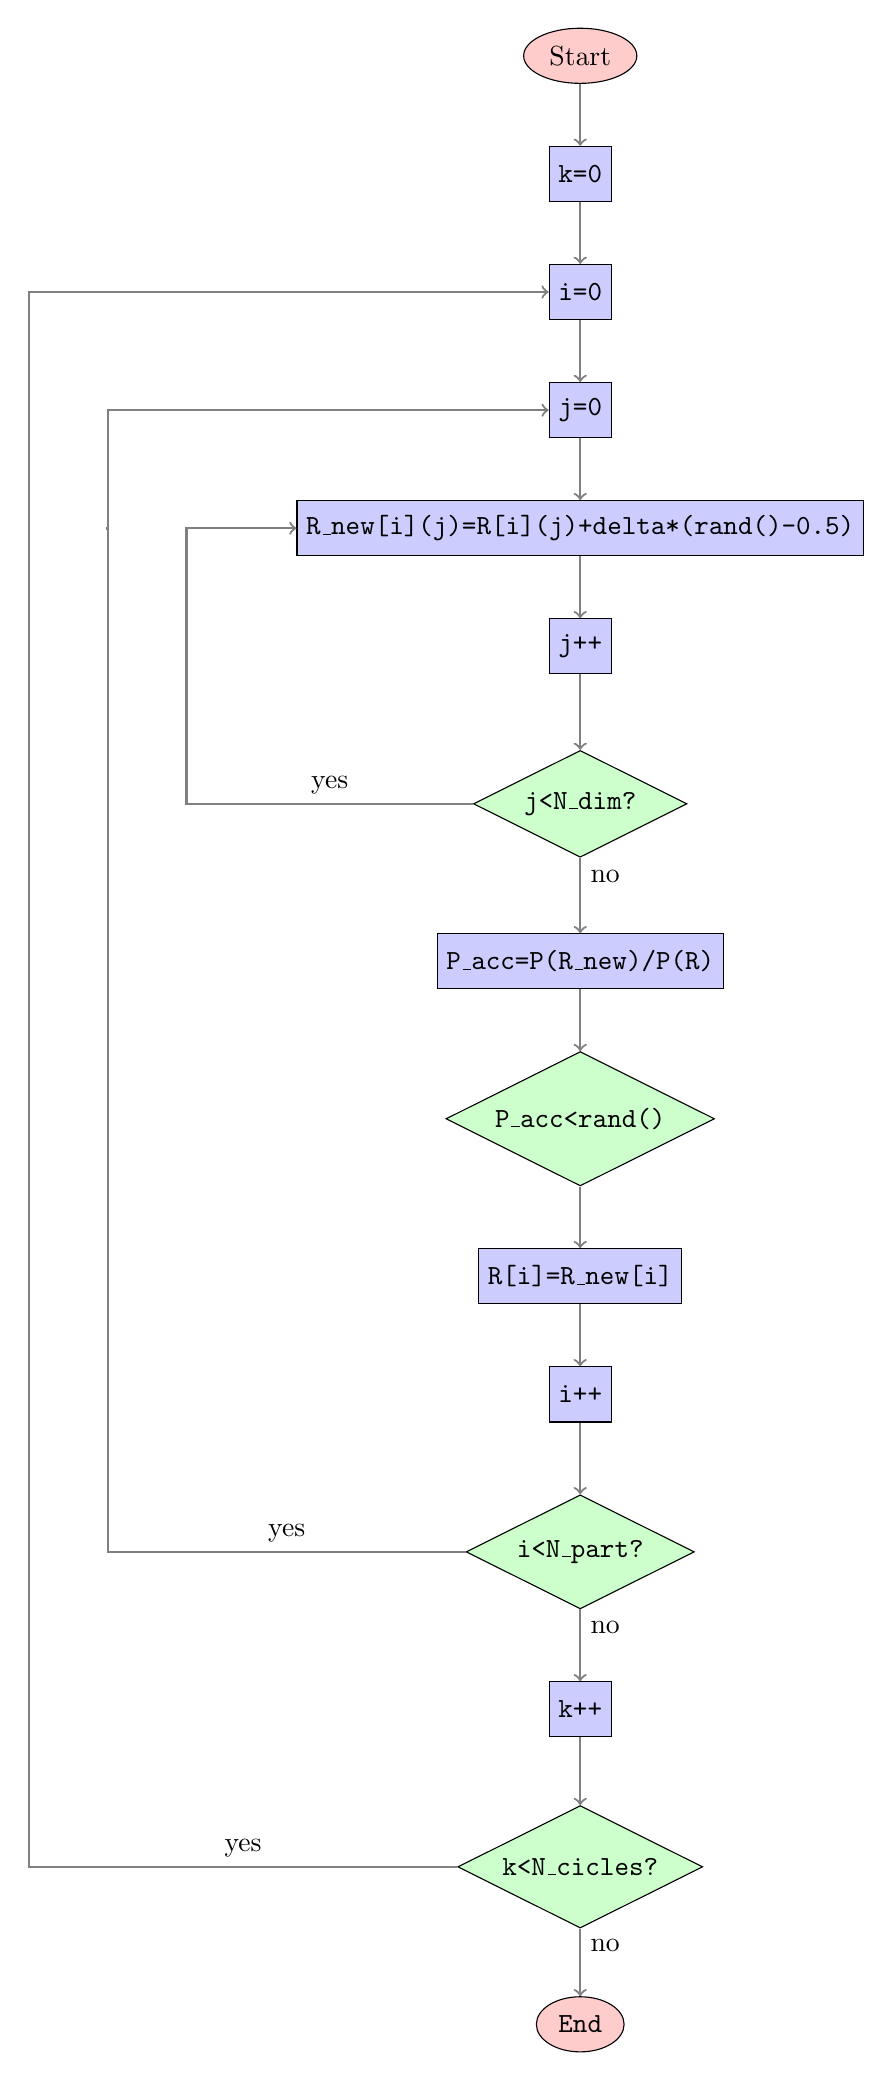
\begin{tikzpicture}[scale=0.5] 

  \node[cloud] (start) {Start};
  \node[block,below of=start] (kinit) {\texttt{k=0}};
  \node[block,below of=kinit] (iinit) {\texttt{i=0}};
  \node[block,below of=iinit] (jinit) {\texttt{j=0}};
  \node[block, below of=jinit] (attempt) {\texttt{R\_new[i](j)=R[i](j)+delta*(rand()-0.5)}};
  \node[block, below of=attempt] (addj) {\texttt{j++}};
  \node[decision, below of=addj] (fordimensions) {\texttt{j<N\_dim?}};
  \node[block, below of=fordimensions, node distance=2cm] (pacc) {\texttt{P\_acc=P(R\_new)/P(R)}};
  \node[decision, below of=pacc] (choose) {\texttt{P\_acc<rand()}};
  \node[block, below of=choose, node distance=2cm] (change) {\texttt{R[i]=R\_new[i]}};
  \node[block, below of=change] (addi) {\texttt{i++}};
  \node[decision, below of=addi] (forparticles) {\texttt{i<N\_part?}};
  \node[block, below of=forparticles, node distance=2cm] (addk) {\texttt{k++}};
  \node[decision, below of=addk] (forcicles) {\texttt{k<N\_cicles?}};
  \node[cloud, below of=forcicles, node distance=2cm] (end) {\texttt{End}};

  \path[arrow] (start)--(kinit);
  \path[arrow] (kinit)--(iinit);
  \path[arrow] (iinit)--(jinit);
  \path[arrow] (jinit)--(attempt);
  \path[arrow] (attempt)--(addj);
  \path[arrow] (addj)--(fordimensions);
  \path[arrow] (fordimensions) -- node[answer,right] {no} (pacc);
  \path[arrow] (pacc)--(choose);
  \path[arrow] (choose)--(change);
  \path[arrow] (change)--(addi);
  \path[arrow] (addi)--(forparticles);
  \path[arrow] (forparticles) -- node[answer,right] {no} (addk);
  \path[arrow] (addk)--(forcicles);
  \path[arrow] (forcicles) -- node[answer,right] {no} (end);

  \node[fake,left of=attempt, node distance=5cm] (pointdim) {};
  \node[fake,left of=pointdim] (pointpart) {};
  \node[fake,left of=pointpart] (pointcicles) {};

  \path[line] (fordimensions) -| node[answer,above] {yes} (pointdim);
  \path[arrow] (pointdim) -- (attempt);
  \path[line] (forparticles) -| node[answer,above] {yes} (pointpart);
  \path[arrow] (pointpart) |- (jinit);
  \path[line] (forcicles) -| node[answer,above] {yes} (pointcicles);
  \path[arrow] (pointcicles) |- (iinit);

 \end{tikzpicture}

\end{document}
